In this chapter we will concern development of basic \textbf{useful}
software program, that utilizes versatility of RexIO library. It will
be an ,,online chat'' program accessed by TELNET.
\index{chat}
\index{online}
\begin{figure}[H]
  \begin{center}
    \leavevmode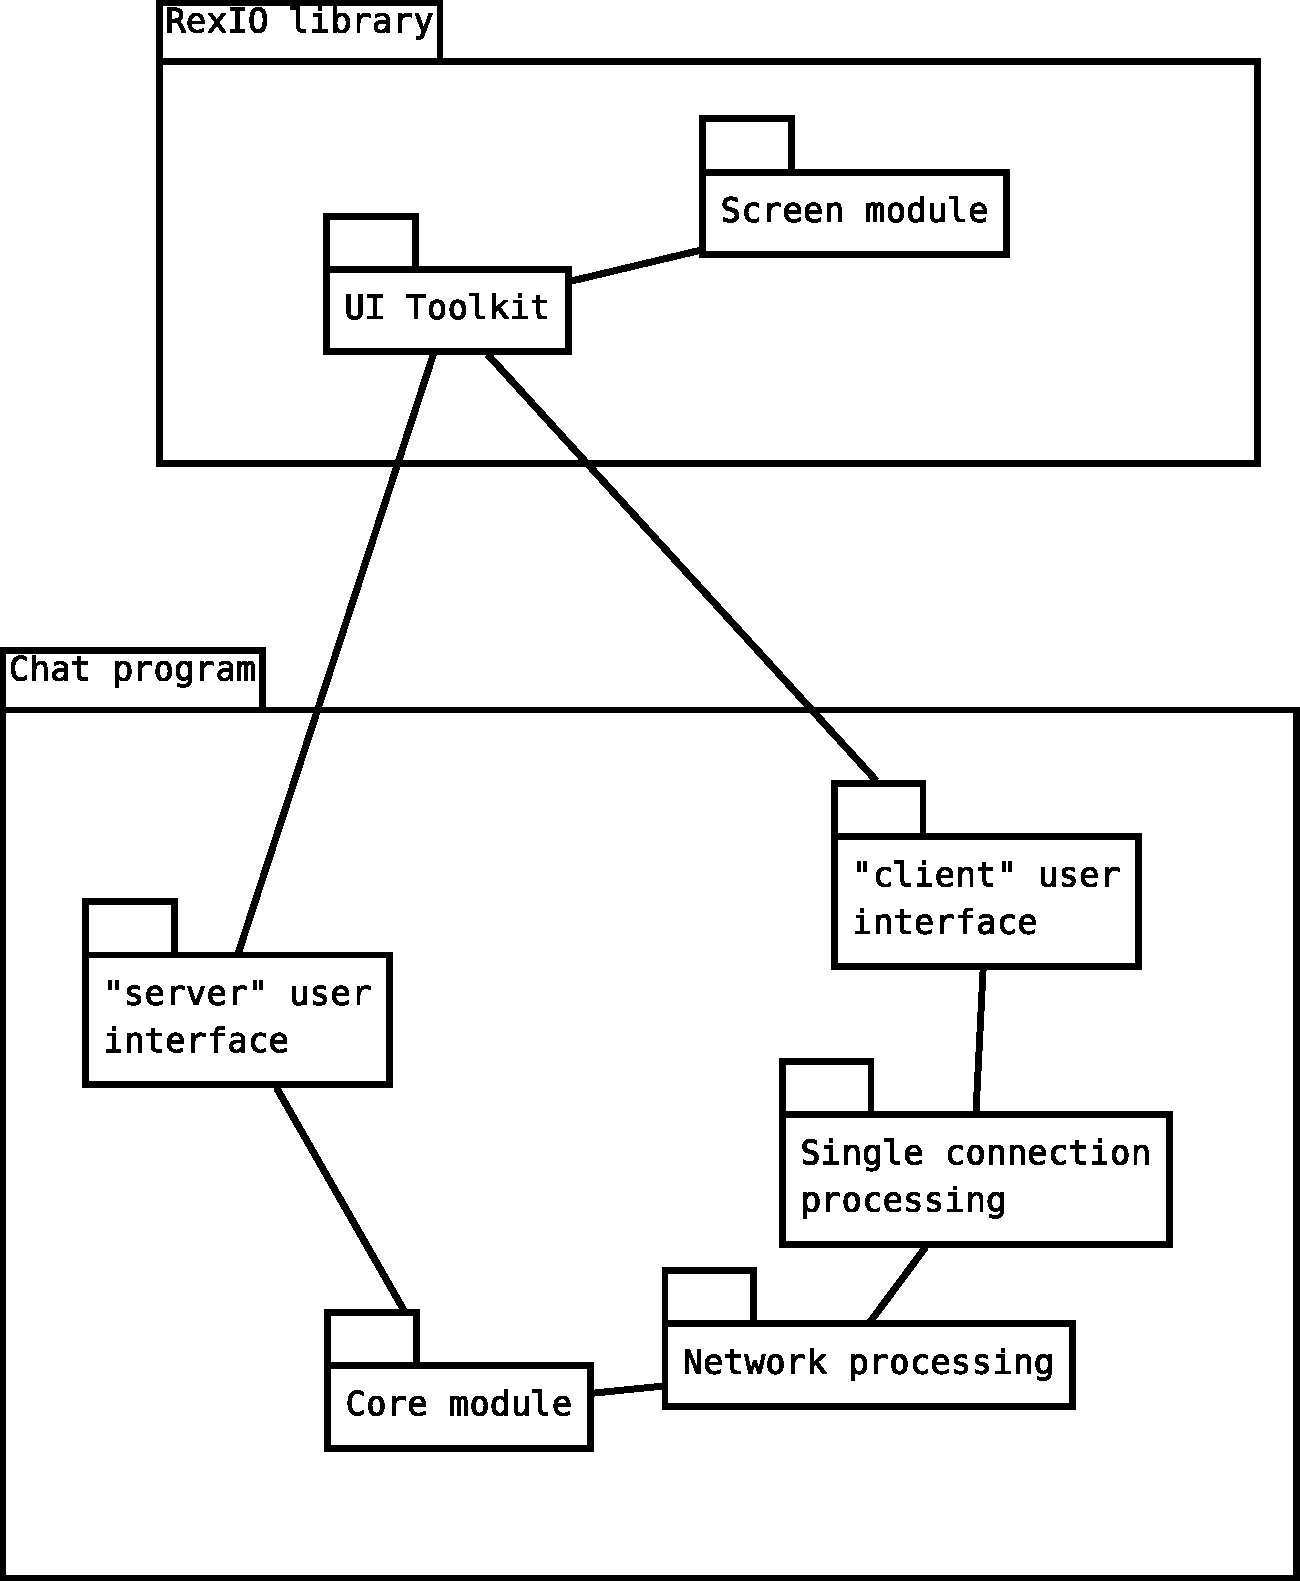
\includegraphics[width=280pt]{graphics/ChatProgram}
  \end{center}
\end{figure}

To run program type for example:
\begin{verbatim}
./test/5/bin/test  -style=test/5/style.rxs -port=4555
\end{verbatim}
  
\verb -style option specifies resource file to be used while
processing connections. This resource file specifies not only colours
of widgets, but also textual values, so it may be used for
internationalization. 

\fullcode
\subsection{Example program listing}
In RexIO distribution this program is located in test/5 directory
\subsubsection{include/main.h++}
\lstinputlisting{../../test/5/include/main.h++}


\subsubsection{include/manager.h++}
\lstinputlisting{../../test/5/include/manager.h++}

\subsubsection{include/demo.h++}
\lstinputlisting{../../test/5/include/demo.h++}


\subsubsection{include/netconn.h++}
\lstinputlisting{../../test/5/include/netconn.h++}


\subsubsection{src/main.c++}
\lstinputlisting{../../test/5/src/main.c++} 


\subsubsection{src/manager.c++}
\lstinputlisting{../../test/5/src/manager.c++}

\subsubsection{src/demo.c++}
\lstinputlisting{../../test/5/src/demo.c++}


\subsubsection{src/netconn.c++}
\lstinputlisting{../../test/5/src/netconn.c++}


\subsubsection{src/netconn.c++}
\lstinputlisting{../../test/5/src/netconn.c++}

\subsubsection{style.rxs}
\begin{verbatim}
RootWindow {
    style: Black Dark Green;
}

FramedWindow {
    style: Red Bright Black;
    frameColor: White Dark Red;
}

LoginWindow {
    style: Red Bright Black;
    frameColor: White Dark Red;
}

Label#welcome {
    style: Yellow Bright Transparent;
    content: "Witaj w aplikacji testowej RexIO";
}

Label#welcome2 {
    style: Yellow Bright Transparent;
    content: "Witaj w aplikacji do pogawędek RexIO!";
}

Inputbox#nickinput {
    style: White Dark Blue;
    cursorStyle: Yellow Bright Yellow;
    activeStyle: White Bright Blue;
}

Button#okbutton {
    style: White Dark Blue;
    activeStyle: White Bright Blue;
}

Label#info0 { content: "Demo to ukazaje działanie RexIO na przykładzie";}
Label#info1 { content: "sieciowej aplikacji do pogawędek.";}
Label#info2 { content: "Interfejs graficzny udostępniany jest przez";}
Label#info3 { content: "zwykły klient "telnet".";}
Label#info5 { style: Magenta Bright Transparent; }
Label#info6 { content: "Użyj telnet by połączyć się z powyższym portem.";}

Label#info15 { content: "Miłego użytkowania!"; }

Label#rexio1 { content: "RexIO jest biblioteką kontroli interfejsu";}
Label#rexio2 { content: "tekstowego z wsparciem dla szerokiej gamy";}
Label#rexio3 { content: "terminali oraz sposobów łączenia. Terminale";}
Label#rexio4 { content: "zdalne jak i lokalne obsługiwane są przez";}
Label#rexio5 { content: "klasy o takim samym interfejsie.";}

RexLogo { style: Cyan Bright Transparent; }

Label#infobar {
    style: White Bright Yellow;
}

Inputbox#msginput {
    style: White Dark Blue;
    cursorStyle: Yellow Bright Yellow;
    activeStyle: White Bright Blue;
}

NickList {
    style: Yellow Bright Red;
    nickColor: Magenta Bright Transparent;
}
\end{verbatim}



\pagebreak
\subsection{Screenshots}
  \index{screenshot}
Server welcome screen
  \begin{figure}[H]
  \begin{center}
  \leavevmode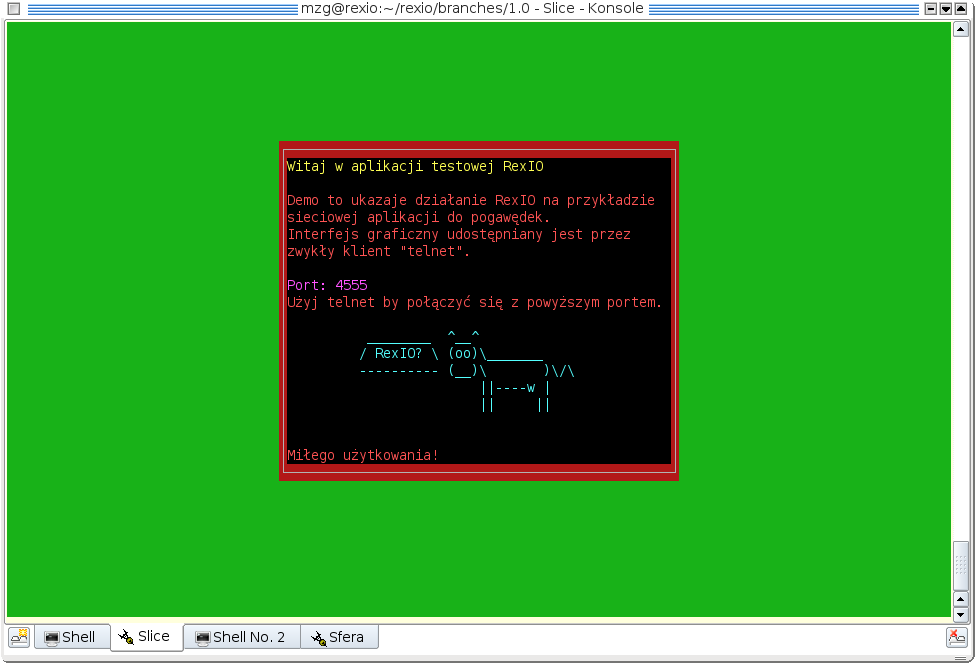
\includegraphics[width=320pt]{graphics/ChatServer}
  \end{center}
  \end{figure}


Client welcome screen
  \begin{figure}[H]
  \begin{center}
  \leavevmode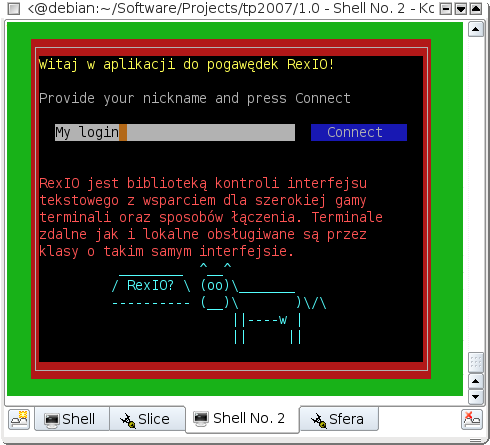
\includegraphics[width=270pt]{graphics/ChatLogin}
  \end{center}
  \end{figure}

\pagebreak
  \index{screenshot}
Client default chat screen
  \begin{figure}[H]
  \begin{center}
  \leavevmode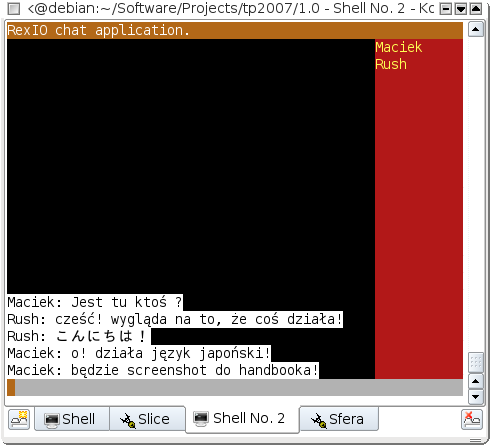
\includegraphics[width=270pt]{graphics/Chat}
  \end{center}
  \end{figure}
